\documentclass[conference,letterpaper,10pt]{IEEEtran}
\usepackage{blindtext, graphicx, url, paralist}

% Add the compsoc option for Computer Society conferences.
%
% If IEEEtran.cls has not been installed into the LaTeX system files,
% manually specify the path to it like:
% \documentclass[conference]{../sty/IEEEtran}

% *** GRAPHICS RELATED PACKAGES ***
%
\ifCLASSINFOpdf
  % \usepackage[pdftex]{graphicx}
  % declare the path(s) where your graphic files are
  % \graphicspath{{../pdf/}{../jpeg/}}
  % and their extensions so you won't have to specify these with
  % every instance of \includegraphics
  % \DeclareGraphicsExtensions{.pdf,.jpeg,.png}
\else
  % or other class option (dvipsone, dvipdf, if not using dvips). graphicx
  % will default to the driver specified in the system graphics.cfg if no
  % driver is specified.
  % \usepackage[dvips]{graphicx}
  % declare the path(s) where your graphic files are
  % \graphicspath{{../eps/}}
  % and their extensions so you won't have to specify these with
  % every instance of \includegraphics
  % \DeclareGraphicsExtensions{.eps}
\fi
%
\usepackage{microtype}

\usepackage{subfigure}
\usepackage{fixltx2e}

\usepackage{multirow}

\usepackage{algorithm2e}
% \usepackage{algorithm}
\usepackage{algorithmic}
\usepackage{xcolor}
\newcommand\todo[1]{\textcolor{red}{#1}}

\hyphenation{op-tical net-works semi-conduc-tor}

\newcommand\adv{$\mathcal{A}$}

\newtheorem{definition}{\textbf{Definition}}[section]
\newtheorem{theorem}{\textbf{Claim}}[section]
\newtheorem{corollary}{\textbf{Corollary}}[theorem]
\newtheorem{lemma}[theorem]{\textbf{Lemma}}

\begin{document}

\title{Namespace Tunnels in Content-Centric Networks}

\author{
\IEEEauthorblockN{Ivan Oliviera Nunes, Gene Tsudik, Christopher A. Wood$^+$ \thanks{$^+$Supported by the NSF Graduate Research Fellowship DGE-1321846.}}
\IEEEauthorblockA{University of California Irvine \\
\{inunes, gene.tsudik, woodc1\}@uci.edu}
}

\maketitle


\begin{abstract}
Content Centric Networking (CCN) is a future Internet architecture which is envisioned as
an alternative to the current IP-based model. CCN emphasizes content distribution by making
contents directly addressable in a request-based information centric network. An advantage
of CCN is that it has some innate privacy friendly features, such as lack of source and
destination addresses in packets. However, to be considered a viable future Internet
architecture, CCN must offer services for private and anonymous communication that are
at least equivalent to those present in the IP architecture. Among such, VPNs are a very
popular application that enables users to send and receive data across shared or public
networks as if their computing devices were directly connected to the same private
network. In this work we design, implement and evaluate CCVPN, a content centric
virtual private network capable of providing the same functionality of VPNs within
the CCN Internet architecture. To the best of our knowledge CCVPN is the first proposal
of a VPN alike service for CCNs. In addition to the CCVPN design, we also provide a
security analysis and experimental performance evaluation for this new system.
\end{abstract}

\begin{IEEEkeywords}
Content-Centric Networking, VPN, Tunneling
\end{IEEEkeywords}

\IEEEpeerreviewmaketitle

\section{Introduction}

\nocite{adams1995hitchhiker}

Ideas:
\begin{enumerate}
  \item \emph{krb-ccn} decouples authentication from access control because access rights
	are not associated with the possession of a key not to the ability of decrypting a
	the content's ciphertext (as in attribute-based encryption). Therefore, access control
	policies can be changed without the need to proactively re-distribute access keys.
  \item Users's privacy is preserved since the actual content producers are not aware of which
	is requesting a given content. This is possible because authentication and AC is handled
	by the KDC and not by the final content producer and because of the lack of source addresses
	on CCN interests.
  \item By leveraging the sinenergy between network names in CCN and Kerberos service-names-based AC, we are
	able to provide an effective AC policy by granting AC rights to namespaces (e.g., \emph{/uci/edu/filesystem/userA/*}).
	In IP Kerberos such AC policies are bounded to principals, with are basically names to services within an organization.
	Since in CCN all content is named by design, \emph{krb-ccn} eliminates the need for principals, leading to a cleaner and
	straightforward authentication and authorization system.
  \item \emph{krb-ccn} is also designed with efficiency in mind. As in IP Kerberos, the majority of cryptografic operations in the
	system consist on symmetric-key authenticated encryption. By avoiding computatially expensive operations (sucha as ABC, PKC, and Pairing Based Cryptography),
	\emph{krb-ccn} becomes suitable for scenarios where content producers are resource constrained devices, such as in an evetual CCN-IoT.
  \item The consumer application does not have to be aware of \emph{krb-ccn}. Based on the interest hierarchical name structure,
	the \emph{krb-ccn} local client is capable of fetching the apropriate TGS/TGT, or issue TGS and TGT requests as needed.
\end{enumerate}


Content-Centric Networking (CCN) is an emerging paradigm that emphasizes the transfer
of named data instead of hosts and interfaces. This shifts the security focus from
channels a la protocols such as TLS to the content itself. If content is sensitive
and must be protected, the architecture demands that it be properly encrypted so
that unauthorized consumers cannot view the data. Access control in CCN has been
well studied in recent years. The majority of solutions rely on long-lived public
and private key pairs to protect data. Specifically, data owners or producers
encrypt data under some access control policy with a public key corresponding to
an authorized consumer (or set of consumers). The recipient(s) use their
corresponding private key to decrypt the content.

In principle, this design achieves its goal of providing access control to content.
However, it suffers in two critical problems. The first is revocation. There is an
intrinsic time-of-check versus time-of-use problem with the standard CCN access
control strategy. Specifically, once content is encrypted under a recipient’s
public key, said recipient will always have access to the data barring destruction
of the private key. If a consumer’s access control rights change after content
is published, then said consumer can continue reading the data so long as it can
obtain an encrypted copy. Addressing this problem requires that access to content
always be preceded by an \emph{online} authorization check. Specifically, before
consumer $Cr_i$ accesses content $C(N)$ with name $N$, it must first acquire access
to $C(N)$. Such access will allow $Cr_i$ to read $C(N)$. Moreover, since access to
$C(N)$ at time $t$ might be allowed for $Cr_i$ but not $Cr_j \not= Cr_i$, $C(N)$ must
only be accessible by $Cr_i$. Generalizing this further means that each content is
uniquely encrypted, on demand, for each consumer at time $t$. Thus, encrypted content
must be bound to the state of an access control policy. Otherwise, caching this
content is, in theory, not possible.

The second critical problem is the inadvertent mixing of authentication and authorization.
In the standard approach, there is not online authentication or authorization. Possession
of a private key sufficiently satisfies both purposes. It is up to the producer to
statically enforce its authorization rules by only encrypting content for particular
consumers. This mixture of authentication and authorization is problematic for several
reasons. Firstly, it binds authorization rules to authentication identities. In
applications where authorization checks depend on more than a client identity, this is
not sufficient. Secondly, it requires that authentication be done solely by consumer-owned
private keys. In fact there are many circumstances where a client’s identity is ascertained
using information that is not a private key — passwords being the more prominent counter
example. In summation, it is advantageous to decouple authentication and authorization,
even in CCN. Kerberos is one system that allows us to partly address both of these open
problems. Specifically, Kerberos decouples authentication and authorization services
through the usage of tickets. It also allows services, e.g., content repositories, to
be accessed over an ephemeral session. Tickets permit the service to check the liveness
of authentication information and, therefore, limit the window of data use beyond revocation.

In this paper, we present Hydra, a system inspired by Kerberos for online access control
enforcement in CCN. Hydra separates consumer authentication and authorization into
separate services. It uses tickets or cookies to allow consumers to convey authorization
permissions to target servers, e.g., content repositories. Servers can use these cookies
to determine if requested content should be provided or not. Hydra also introduces a
novel naming scheme to bind consumer credentials to protected content objects. This
allows only authorized consumers to derive the names of protected content objects.
Producers use these derived names when checking authorization rights for target content
or namespaces. This naming scheme is orthogonal to Hydra and may be used in other
application settings to better make access control decisions.

\section{Preliminaries}\label{sec:prelims}
This section presents an overview of the CCN architecture\footnote{Named-Data Networking \cite{jacobson2009networking}
is an ICN architecture related to CCN. However, since CCNxKE was
designed for ICNs that have features which are not supported by NDN (such
as exact name matching), we do not focus on NDN in this work. However,
CCNx could be retrofitted to work for NDN as well.} and work
related to confidentiality, privacy, and transport security. Those familiar with these topics
can skip it without loss of continuity.

\subsection{CCN Overview}
In contrast to IP networks, which focus on end-host names and addresses,
CCN \cite{jacobson2009networking,mosko2016semantics} centers
on content by making it named, addressable, and routable within the network. A
content name is a URI-like string composed of one or more
variable-length name segments, each separated by a \url{`/'} character. To
obtain content, a user (consumer) issues a request, called an \emph{interest}
message, with the name of the desired content. This interest can be
\emph{satisfied} by either (1) a router cache or (2) the content producer. A
\emph{content object} message is returned to the consumer upon satisfaction of
the interest. Moreover, name matching in CCN is exact, e.g., an interest for
\url{/edu/uci/ics/cs/fileA} can only be satisfied by a content object
named \url{/edu/uci/ics/cs/fileA}.

In addition to a payload, content objects include several fields. In this work,
we are only interested in the following three: {\tt Name}, {\tt Validation}, and {\tt ExpiryTime}.
The {\tt Validation} field is a composite of (1) validation algorithm information
(e.g., the signature algorithm used, its parameters, and a link to the public
verification key), and (2) validation payload (e.g., the signature). We use the
term ``signature'' to refer to this field. {\tt ExpiryTime} is an optional,
producer-recommended duration for the content objects to be cached.
Conversely, interest messages carry a mandatory name, optional payload, and
other fields that restrict the content object response. The reader is encouraged
to review \cite{mosko2016semantics} for a complete description of all packet fields
and their semantics.

Packets are moved in the network by routers or forwarders. A forwarder is composed
of at least the following two components:
\begin{compactitem}
\item {\em Forwarding Interest Base} (FIB) -- a table of name prefixes and
  corresponding outgoing interfaces. The FIB is used to route interests based on
  longest-prefix-matching (LPM) of their names.
\item {\em Pending Interest Table} (PIT) -- a table of outstanding (pending)
  interests and a set of corresponding incoming interfaces.
\end{compactitem}
%
A forwarder may also maintain an optional {\em Content Store} (CS) used for content
caching. The timeout for cached content is specified in the \texttt{ExpiryTime}
field of the content header. From here on, we use the terms {\em CS} and
{\em cache} interchangeably.

Forwarders use the FIB to move interests from consumers towards producers and the PIT
to forward content object messages along the reverse path towards consumers. More
specifically, upon receiving an interest, a router $R$ first checks its cache
(if present) to see if it can satisfy this interest locally. If the content is
not in the cache, $R$ then consults the PIT to search for an outstanding
version of the same interest. If there is a PIT match, the new incoming interface
is added to the PIT entry. Otherwise, $R$ forwards the interest to the next hop
according to its FIB (if possible). For each forwarded interest, $R$ stores
some amount of state information in the PIT, including the name of the interest and the
interface from which it arrived, so that content may be sent back to the
consumer. When content is returned, $R$ forwards it to all interfaces listed in
the matching PIT entry and said entry is removed. If a router receives a content object
without a matching PIT entry, the message is deemed unsolicited and subsequently
discarded.

\section{Related Work} \label{sec:related}

There are generally two classes of related work: (1) anonymity networks, such
as ANDaNA \cite{dibenedetto2011andana} and AC3N \cite{tsudik2016ac3n}, and
(2) encryption-based access control techniques. ANDaNA was developed as a
proof-of-concept application-layer anonymizing network for NDN. It works by
creating single-use, ephemeral, and anonymizing circuits between a consumer
and producer. Each hop in this circuit uses onion decryption to decapsulate
interests and onion encryption to encrypt the result. A minimum of two hops are
needed to guarantee consumer and producer unlinkability. CCVPN seeks to address
a different threat: privacy instead of anonymity. Thus, only a single hop, which
creates a tunnel between a source and a sink AS, is needed in CCVPN. Moreover,
since these tunnels serve multiple traffic flows for \emph{all} consumers within
the same source, they are long-lived and persistent. This reduces the per-packet
and per-flow cryptographic operations needed to move packets between the source
and sink domains. AC3N \cite{tsudik2016ac3n} is an optimized version of ANDaNA
that keeps per-flow state in each hop of an anonymizing circuit to specify
ephemeral key identifiers for packets. This prevents intra-flow linkability
while simultaneously enabling symmetric-key encryption and decryption for more
efficient processing. However, since AC3N is still a per-consumer application,
anonymizing circuits cannot be shared among multiple geolocated consumers
in the same domain.

Content encryption seeks to solve the problem of data confidentiality rather than
privacy or anonymity. This technique allows content to be disseminated throughout
the network, since it cannot be decrypted by adversaries without the appropriate decryption key(s).
Many variations of this approach have been proposed based on general
group-based encryption \cite{Smetters2010}, broadcast encryption \cite{Misra2013,Ion2013}, and
proxy re-encryption \cite{Wood2014}. Kurihara et al. \cite{ifip15} generalized these specialized
approaches in a framework called CCN-AC, an encryption-based access control framework
that shows how to use manifests to explicitly specify and enforce other encryption-based
access control policies. Consumers use information in the manifest to (1) request appropriate
decryption keys and (2) use them to decrypt content object(s). The NDN NBAC \cite{yu2015name}
scheme is similar to \cite{ifip15} in that it allows decryption keys to be
flexibly specified by a data owner. However, it does this based on name engineering rules instead of
configuration. Interest-based access control \cite{ghali2015interest} is a different
type of access control scheme wherein content is optionally encrypted. Access
is protected by making the names of contents derivable only by authorized consumers.
NDN-ACE \cite{shangndn} is a recent access control framework for IoT environments
which includes a key exchange protocol for distributing secret keys to sensors.
All of these techniques, with few exceptions, use public-key cryptographic schemes
to protect only the \emph{payload} of content packets. They do not encapsulate complete
packets for private transmission between a source and sink domain. The exception is CCNxKE~\cite{ccnxke},
which specifies a key exchange protocol that can bootstrap secure sessions between a source
a sink. CCNxKE can be used by CCVPN to establish pairwise shared secrets between tunnel
endpoints, even though this step is not strictly required.

\section{Hydra}

\nocite{adams1995hitchhiker}

%% XXX: show the hydra protocol here..

There are at least two fundamental problems one must address in any access control
system: (1) how access control policies are represented and (2) how they are enforced.
Policy representation specifies how policies are mapped onto resources (or content).
For example, one representation might map content names to sets of public keys. These
keys could be owned by authorized consumers and are used when encrypting content.
Encrypting content with name $N$ under a key $pk$ restricts access to the owner of
the corresponding private key. The challenge is to devise a representation that
scales well with the number of resources (content) and consumers. Regardless of
the approach, we claim there is one fundamental feature that must be present for
every access control decision: consumer requests must be bound to a principal.
This allows the producer or entity serving data to provide the appropriate
representation of the target data to the consumer. To achieve this goal, Hydra
uses AccessIDs described in the previous section.

The second problem is rooted more in system design. Consider what must be done
to satisfy a request for access-controlled content. First, the requestor must
be authenticated to bind the request to a principal. Second, the request must
be authorized to determine if access to the desired content is permissable. Lastly,
the data must be packaged in a protected (encrypted) form for the requestor. Thus,
problem (2) is more about how entities are configured to handle the separate
authentication, authorization, content distribution steps in CCN.

In past work, these roles were often convoluted. In particular, \cite{pre,be}
assumed that the entity which handles data production was also implicitly
responsible for content authentication and authorization. CCN-AC \cite{xx} and
NDN-NBAC \cite{xx} separated the authentication and authorization service from
the data production. Specifically, data owners generate and distribute consumer (principal)
private keys to consumers through out-of-band channels. Data producers receive
the corresponding public keys through a similar channel. These are used to encrypt
randomly generated per-content encryption keys.

Despite this separation, these designs still suffer from the following problems.
{\bf First}, authentication and authorization are unnecessarily coupled, leading
to an inherent ``time of check'' versus ``time of use'' problem. Specifically,
consumers obtain private keys from the data owner at time $t$ and use them to
decrypt content at time $t' > t$. {\bf Second}, if consumers are forced to fetch
their private keys from the data owner, a single point of failure emerges. In
particular, it becomes easy to launch a Denial of Service (DoS) attack on the
data owner by forcing it to perform expensive cryptographic operations, e.g.,
signature verifications.
%% @Ivan, the reasons above are ridiculous -- please add others!

Hydra is a system designed to address these problems. It has the following features:
%
\begin{compactitem}
    \item Consumer authentication and content authorization decisions can be separated
    and performed by separate systems in the network. A Hydra administrator can spawn
    any number of authentication endpoints to handle client authentication requests.
    Consumers are unable to fetch data from the authorization agent without having
    first been authenticated.
    \item Authorization decisions are centralized to a single system (or set of synchronized
    systems). This permits each authorization check to be done in real-time without
    introducing any added delay between the subsequent use.
    \item XXX
    \item XXX
    \item XXX
\end{compactitem}
%

\begin{table*}
\centering
\caption{Notation summary}
\label{notation}
\begin{tabular}{|l|p{6cm}|}
\hline
Notation    			&  Description  							\\ \hline \hline
$I.name$			&  Name of the issued interest I					\\&\\
$N$				&  A namespace prefix (e.g., /uci/ics/ivan/\*) 				\\&\\
$TGT\_Name$			&  Ticket-granting-ticket name (e.g., /uci/ics/TGT) that will be routed towards authenticator \\&\\
$TGS\_Name$			&  Ticket-granting-service name (e.g., /uci/ics/TGS) that will be routed towards authorizer   \\&\\
$sk_C$      			&  Consumer Secret Key						        \\&\\
$pk_C$			        &  Consumer Public Key, including public UID and certificate        	\\&\\
$k_A$ 	   		 	&  Long term symmetric key shared between Authenticator and Authorizer  \\&\\
$k_P$ 	   		 	&  Long term symmetric key shared between Authenticator and Producer    \\&\\
$s \sample \{0,1\}^{\lambda}$	&  Random ${\lambda}$-bits number generation    	     		\\&\\
$ct = Enc_{k}(pt) $		&  Authenticated Encryption of $pt$ using symmetric key $k$		\\&\\
$pt = Dec_{k}(ct) $		&  Decryption of $ct$ using symmetric key $k$    	     		\\&\\
$ct = Enc_{pk}(pt) $		&  Authenticated Encryption of $pt$ using public key $pk$ 		\\&\\
$pt = Dec_{sk}(ct) $		&  Decryption of $ct$ using secret key $sk$    	     			\\&\\
$\sigma = Sign_{sk}(m) $	&  Signature on message $m$ using secret key $sk$ 			\\&\\
$Verif_{pk}(\sigma,m) $		&  Signature verification using public key $pk$     			\\&\\
\hline
\end{tabular}
\end{table*}

\begin{figure*}
\begin{center}
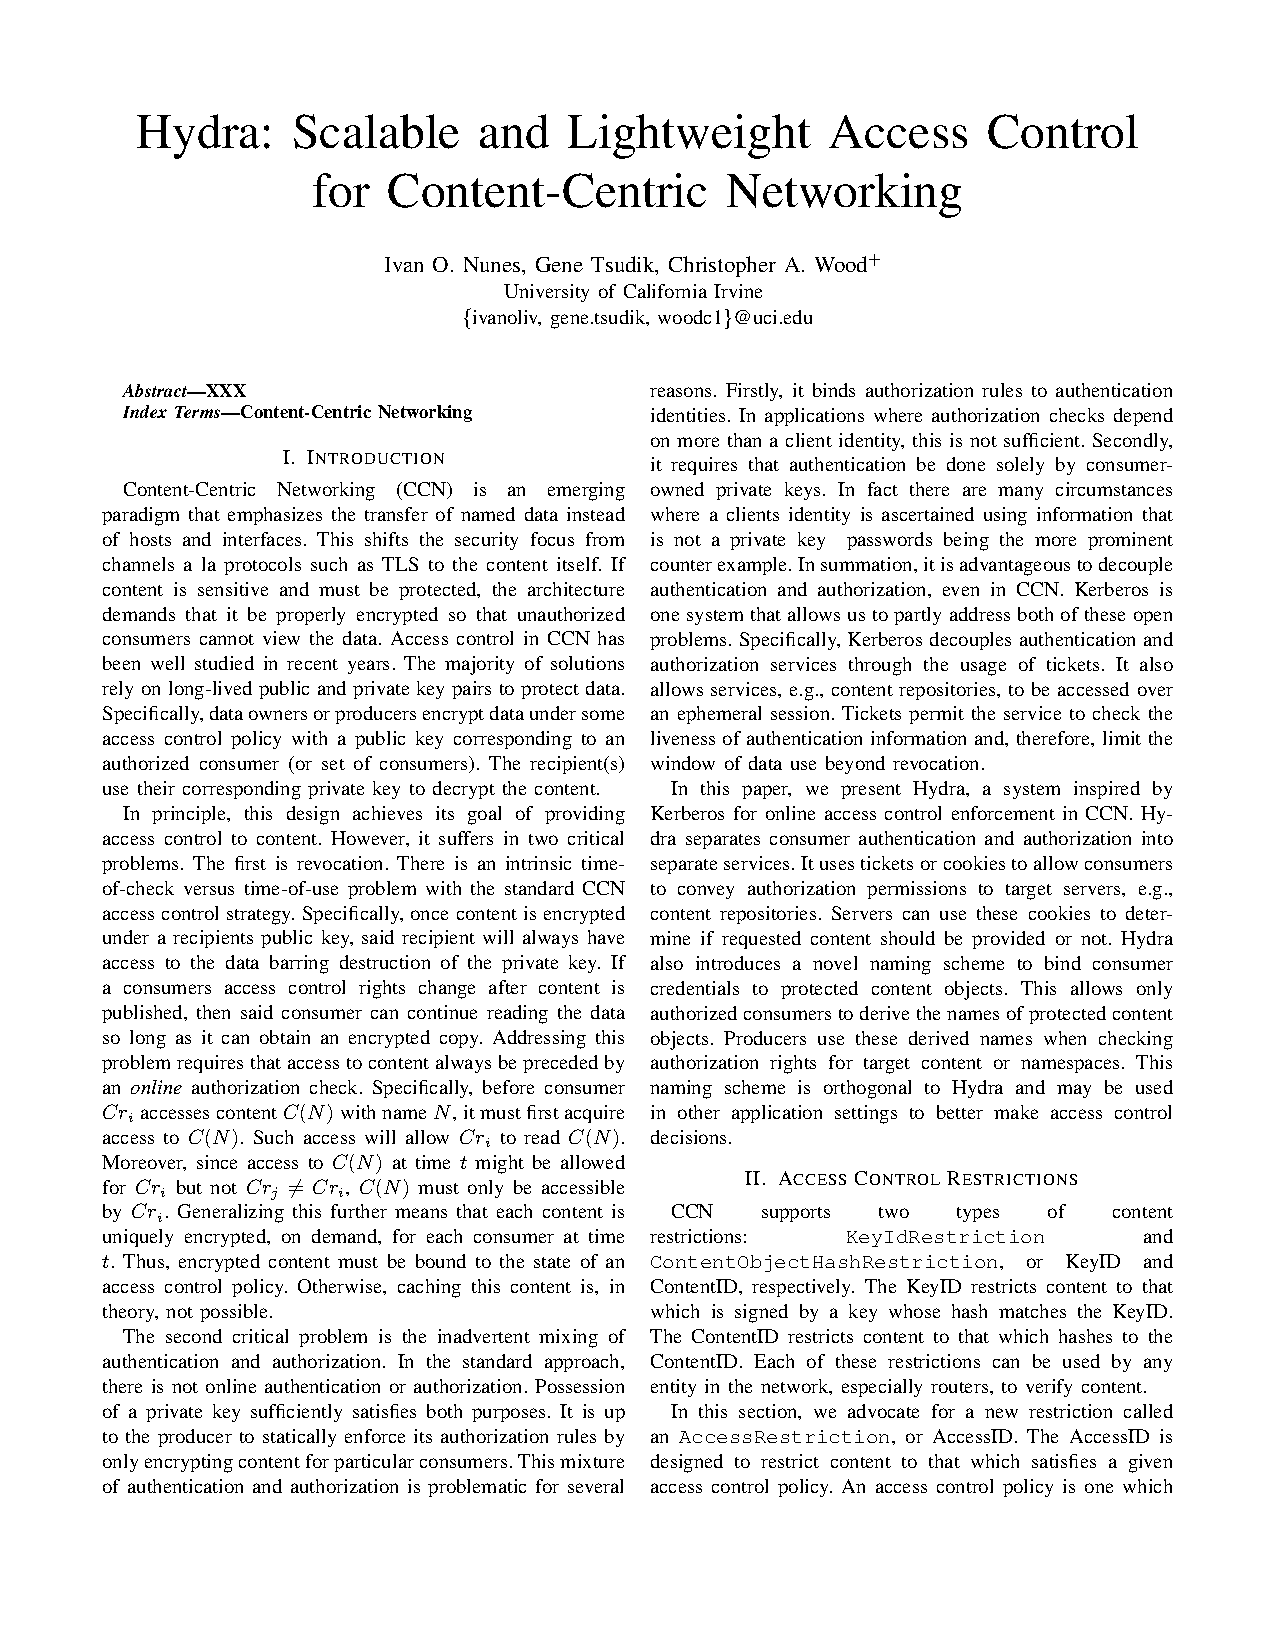
\includegraphics[scale=0.5]{Figures/hydra.pdf}
\caption{Hydra system design}
\label{fig:spectr-basic}
\end{center}
\end{figure*}




\begin{figure*}
\begin{center}
\fbox{
\procedure{}{%
\textbf{Consumer} \> \> \textbf{Authenticator} \\
\mathsf{I.name = TGT\_Name} \> \> \\
\sigma = \mathsf{Sign}_{sk_C}(\mathsf{I.name}) \> \> \\
\> \xrightarrow{payload = \sigma, pk_C} \> \\
\> \> \text{Verify Claimed $pk_C$ UID on users DB} \\
\> \> \mathsf{Verify}_{pk_C}(\sigma,\mathsf{I.name}) \\
\> \> s \sample \{0,1\}^{\lambda} \\
\> \> t = \mathsf{setExpirationTime}() \\
\> \> k_{TGS} \sample \{0,1\}^{\lambda} \\
\> \> \mathsf{token}_{TGS}^{C} \gets \mathsf{Enc}_{pk_C}(k_{TGS}||t) \\
\> \> \mathsf{TGT} = \mathsf{Enc}_{k_{A}}(pk_C || s || t || k_{TGS}) \\
\> \xleftarrow{payload = s, \mathsf{TGT}, \mathsf{token}_{TGS}^{C}} \> \\
k_{TGS},t = \mathsf{Dec}_{sk_C}(\mathsf{token}_{TGS}^{C}) \> \> \\
\mathsf{store(TGT,s,t,k_{TGS})} \> \> \\
}
}
\caption{Consumer authentication protocol}
\label{fig:spectr-basic}
\end{center}
\end{figure*}




\begin{figure*}
\begin{center}
\fbox{
\procedure{}{%
\textbf{Consumer} \> \> \textbf{Authorizer} \\
\mathsf{I.name = TGS\_Name} \> \> \\
\> \xrightarrow{payload=N, s, \mathsf{TGT}} \> \\
\> \> pk_C || s' || t || k_{TGS} = \mathsf{Dec}_{k_{A}}(TGT) \\
\> \> \text{Verify: $s = s'$} \\
\> \> \text{Verify: $t$ not expired} \\
\> \> {k_P} = \mathsf{verifyPolicyAndFetchKey}(N, pk_C) \\ %Kp can be different things (shared key between all boxes that implement that producer, broadcast encryption key, etc)
\> \> k_{N} \sample \{0,1\}^{\lambda} \\
%\> \> r \sample \{0,1\}^{\lambda} \\ why?
\> \> t = \mathsf{setExpirationTime}() \\ %% timestamp
\> \> \mathsf{TGS} \gets \mathsf{Enc}_{k_P}( N || k_N || t) \\ %% encrypt the key in the ticket
\> \> \mathsf{token}_N^{C} \gets \mathsf{Enc}_{k_{TGS}}(k_N||t) \\
\> \xleftarrow{payload=\mathsf{token}_N^{C}, \mathsf{TGS}} \> \\
k_N,t = \mathsf{Dec}_{k_{TGS}}(\mathsf{token}_N^{C}) \> \\
\mathsf{store(N,TGS,t,k_N)} \>
}
}
\caption{Consumer-data authorization protocol}
\label{fig:spectr-basic}
\end{center}
\end{figure*}

\begin{figure*}
\begin{center}
\fbox{
\procedure{}{%
\textbf{Consumer} \> \> \textbf{Producer} \\
\mathsf{I.name = N||suffix} \> \> \\
\> \xrightarrow{payload= TGS} \> \\
\> \>  N' || k_N || t = \mathsf{Dec}_{k_P}(TGS) \\
\> \> \text{Verify: $N'$ is prefix of I.name} \\
%%\> \> \text{Verify: $pk_C'$ = $pk_C$} \\ Not sure this is necessary
\> \> \text{Verify $t$ expiration} \\
\> \> D = \mathsf{ProduceData}(\mathsf{I.name}) \\
\> \> D' = \mathsf{Enc}_{k_N}(D) \\
\> \xleftarrow{payload=D'} \> \\
D = \mathsf{Dec}_{K_N}(\mathsf{D'}) \> \> \\
}
}
\caption{Consumer-data authorization protocol}
\label{fig:spectr-basic}
\end{center}
\end{figure*}

\subsection{Ivan: Comments}
\begin{enumerate}
 \item IMHO, the authentication algorithm (Fig.2) should be unrelated to the namespace you want to get access to. Only related to Consumer's claimed Identity. Otherwise the consumer has to go back to the Authenticator every time she wants a different content (3 RTT).
 \item Unless we are assuming that there is some magical non-deterministic router that will route the same name through different paths, I.name must specify the content produced by the Authenticator, i.e., the TGT. The same applies for TGS.
 \item The TGT as a MAC never expires. My suggestion is to encrypt a timestamp, as in Kerberos, and as we are doing in the authorizer. MAC with an epoch is also an option, but not a good one.
 \item PKE of $K_N$ in the authorization algorithm (Fig 3) could (and maybe should) be symmetric AEAD.
 \item $verifyPolicyAndFetchKey()$ : Could be implemented as broadcast encryption...
 \item Consumer has to receive the expiration date of TGT/TGS. This way Consumer can get back to Authenticator/Authorizer directly, without issuing expired TGT/TGS messages to authorizer/producers.
\end{enumerate}
\section{CCVPN Security}\label{sec:sec-analysis}


\subsection{System and Security Model} \label{sec:goals}

Our security analysis considers the worst case scenario, in which the consumer issues an
interest that has not been cached in any of the routers from the consumer nor producer domains.
Therefore, the interest must traverse the entire network until reaching the producer.
Conversely, the content needs to be forwarded all the way back though the same path
satisfying the routers' PIT entries. A system that is secure in this worst case is also
secure when the content has been previously cached in some router along the way.

\textbf{Adversary Goals and Capabilities.} The goal of the adversary \adv\ is either 1) to
retrieve any information associated with the original issued interest $I_p$ and/or the
original content $C_p$ or 2) to retrieve the identities of the consumer and/or producer,
thus violating the anonymity in the communication. \adv\ is also considered successful
if it is able to impersonate the content producer by faking a content response. Since the
original interest and the original content are visible inside the consumer and producer
domains, we here assume that \adv\ cannot eavesdrop or compromise hosts inside
such domains. It is also worth to emphasize that, by the conceptual design of the VPN,
communication is anonymous to hosts from outside the VPN but not to hosts that belong to
that VPN. Anyhow, one-to-one anonymous communication is still achievable sing the VPN
paradigm if the communication must be anonymous to any other host in the network. This
also means that, as components of the producer and consumer domains, we assume that the
gateways $G_c$ and $G_p$ cannot be compromised.

In our model \adv\ is allowed to perform the following actions (when outside the consumer and producer domains):

\begin{itemize}
	\item \textbf{Eavesdrop and replay traffic:} \adv\ can eavesdrop on a link
    learning among other things the packet contents and traffic patterns.
	\item \textbf{Deploy compromised routers or compromise existing routers:} \adv\ is capable of
    deploying a compromised router ou compromised an existent router outside the VPN domains. By doing
    so \adv\ becomes capable of maliciously injecting, delaying, altering, and dropping traffic.
    In addition, when an existing router is compromised, \adv\ learns all of the private
    information contained in that router, such as private keys and cached content.
	\item \textbf{Deploy compromised caches:} As a consequence of the ability to compromise and
    deploy compromised routers, \adv\ is also able to deploy compromised caches. This
    includes monitoring the routers' cache contents and replying with corrupted or fake data.
\end{itemize}

\subsection{Additional Considerations}

\textbf{Gateway-to-Gateway Authentication:} At this point one might have noticed that,
in the CCVPN design, any host that possesses the producer -side gateway ($G_p$) public-key
is able to initiate an anonymous communication link with $G_p$. In other words, the design
does not include any authentication between the consumer-side gateway $G_c$ and $G_p$.
Indeed, authentication is not required in CCVPN because is in not needed in some application scenarios.

Suppose, for instance, that a content provider offers its contents to any host in the Internet
but it also  wants such hosts to be able to anonymously request and receive such content. In
this case, since any host in the Internet should be able to requests the contents, there is no
need for the consumer-side $G_c$ to authenticate it self to $G_p$.

Another use case for CCVPN is the traditional VPN use case, in which two physically separated
local networks (for instance, offices of the same company in different countries) should virtually
behave as a private local network. In that case, it is necessary to prevent that a given $G_c$,
which is not part of that corporation's network to connect to $G_p$ and become part of the VPN.
To that purpose, standard host-to-host CCN authentication mechanisms can be used to authenticate
$G_p$ and $G_c$ to each other. This must be performed before any VPN communication, to make sure
that only the appropriate parties are communicating under the CCVPN architecture. We leave the
evaluation and specification of gateway-to-gateway authentication protocols as future work (see Sec.~\ref{sec:conclusion}).

\textbf{Denial of Service:} Since CCVPN gateways are connected to the public network they are
clearly susceptible to DoS attacks. In the CCVPN architecture, both $G_c$ and $G_p$ are
susceptible to DoS attacks. A DoS attack on $G_p$ would consist in flooding it with several
fake encapsulated interests. Conversely, a DoS attack on $G_c$ would basically consist
of flooding it with an enormous amount of encrypted content packets. In the case of $G_p$,
such attacks are specially harmful since the interest decapsulation involves a public-key
decryption operation. We plan to consider DoS countermeasures in future work.

\subsection{Security Analysis}

In this section we analyze the security of CCVPN. Our main security goal is
preventing \adv\ from achieving any of the goals outlined in Section \ref{sec:goals}.
Formally, this translates into semantic security of all traffic, modulo what can be inferred via traffic analysis.
A consequence of this property is that an off-path adversary, i.e., one that is
not in the consumer or producer domain, is unable to forge packets with
non-negligible probability. Our analysis relies on arguments in the standard
security model. It consists of assessing the security of the interest and
content encapsulation algorithms.

\begin{definition}\label{def1}
\textit{
An interest encapsulation algorithm $Encapsulate(I_p)$ is an indistinguishable
interest encapsulation iff, given any two interests $I_p^1$ and $I_p^2$, chosen
by the adversary, and a randomly selected bit $b$, the adversary has only $1/2 + \epsilon$
probability of guessing the value of the bit $b$ when given $I_e^b = Encapsulate(I_p^b)$.
Where $\epsilon$ is a negligible factor with regard to the security parameter $k$.
}
\end{definition}

\begin{theorem}\label{theo1}
\textit{
Let $Encapsulate_{pk}(I_p)$ denote the interest encapsulation routine described in
Algorithm~\ref{alg:interestEncap}. If $Enc_{pk}$, used to construct $Encapsulate_{pk}(I_p)$,
is a CPA-secure public-key encryption scheme then $Encapsulate_{pk}(I_p)$ is an
indistinguishable interest encapsulation algorithm.
}
\end{theorem}

\textit{\textbf{Proof--}} Suppose that Claim~\ref{theo1} is false. Then there exists a
polynomial adversary $Adv$ capable of guessing the bit $b$ of Definition~\ref{def1}
with non-negligible advantage, when given $I_e^b = Encapsulate(I_p^b)$ with
$b \leftarrow \{0,1\}$ chosen at random. We show that if such adversary exists he can
be used to construct a polinomial adversary $AdvCPA$ which breaks the CPA-security
of $Enc_{pk}$. $AdvCPA$ plays the CPA-security game with a challenger sending him
two messages $m^0$ and $m^1$. Following the CPA-security game, the challenger
randomly chooses a value for the bit $b' \leftarrow \{0,1\}$ and gives back
$C = Enc_{pk}(m^{b'})$ to $AdvCPA$. To break the CPA-security $AdvCPA$ must be
able to guess the value of the bit $b'$ with non-negligible advantage. To that
purpose $AdvCPA$ can query the challenger for the encryptions of $m^0$ and
$m^1$ ($c^0 = Enc_{pk}(m^0)$ and $c^1 = Enc_{pk}(m^1)$) and then construct two
interests $I_e^0 = createNewInterest(Gp_{name}, c^0)$ and $I_e^1 = createNewInterest(Gp_{name}, c^1)$,
using the same $createNewInterest$ function used by algorithm~\ref{alg:interestEncap},
which is public (notice that $Gp_{name}$ is also public). Finally, $AdvCPA$ gives $I_e^0$
and $I_e^1$ as input to $Adv$ and outputs whatever $Adv$ outputs. Since under our
assumption $Adv$ guesses the bit $b$ with non-negligible advantage, then $AdvCPA$ breaks
the CPA-security of $Enc_{pk}$. But this violates the hypothesis of Claim~\ref{theo1}
and, therefore, such $Adv$ cannot exist.

\begin{definition}
\textit{
A content encapsulation algorithm $Encapsulate(C_p)$ is an indistinguishable content
encapsulation iff, given any two contents $C_p^1$ and $C_p^2$, chosen by the adversary,
and a randomly selected bit $b$, the adversary has only $1/2 + \epsilon$ probability
of guessing the value of the bit $b$ when given $C_e^b = Encapsulate(C_p^b)$. Where
$\epsilon$ is a negligible factor with regard to the security parameter $k$.
}
\end{definition}

\begin{theorem}
\textit{
Let $ContentEnc_{k_r}(C_p)$ denote the content encapsulation routine described in
Algorithm~\ref{alg:contentEnc}. If $EncryptThenMAC_{k_r}$, used to construct
$ContentEnc_{sk}$, is a CCA-secure symmetric-key encryption scheme, then:
\begin{enumerate}
\item $ContentEnc_{k_r}(C_p)$ is an indistinguishable content encapsulation algorithm;
\item An adversary has only negligible probability of generating a valid fake encapsulated content $I_c'$
\end{enumerate}
}
\end{theorem}

\textit{\textbf{Proof (Sketch)--}} This follows directly from the definition of
CCA-security and from the same argument in the previous proof.

\section{Performance Analysis}\label{sec:analysis}

In this section we analyze and discuss the overhead of the CCVPN design with respect
to the additional processing time and state consumption needed to handle traffic.

\subsection{State Consumption}
The CCVPN design has an immediate impact on the FIB and PIT size of a gateway.
(The content store size remains unaffected since only decapsulated content objects
are ever cached.) Let $F_S$ be the total size of a standard forwarder
FIB in terms of bytes and
$N_F$ be the number of entries in the FIB. For simplicity, we will assume that
each name prefix in the FIB has a constant size of $64$B. In practice we expect
this to be a comfortable upper bound. Thus, $F_S = N_Fs$, where $s$ is the size of
each FIB entry. Here, $s$ includes a name prefix (of size $64$B) and a bit vector
that identifies the matching links for the interface. We assume that a gateway has
$128$ links which, again, is a comfortable upper bound. Therefore, $F_S = 80N_F$B.
Now consider the FIB size $F_G$ for a CCVPN gateway. Some entries in these FIBs will
point to ``private'' prefixes, i.e., other domains, and therefore have a larger size
to account for the corresponding prefix and key material that must be stored.
For both public- and symmetric-key encryption, the key size is the same: $32$B \cite{sodiumGithub}.
Therefore, by taking into account two both the FIB entry prefix key, translation
prefix, encryption key, and corresponding bit vector, the total size of one ``private''
FIB entry will be $176$B, meaning that $F_G = 176N_F$B. By comparing $F_S$ to $F_G$, we
see that, in the worst case, the CCVPN FIB is at most $F_G/F_S = 176/80 = 2.2$ times larger
than the standard FIB. In practice, however, we expect this to be much smaller, since the
fraction of public to private FIB entries in a gateway will be non-zero.

We will now apply the same analysis to the PIT size. A standard PIT entry includes a
complete name and ingress bit vector. (They may also include the optional {\tt KeyId}
and {\tt ContentId}, but since they are included in the gateway PIT as well we omit them
from this analysis.) A gateway PIT entry will contain the same elements of a standard
PIT entry but also a symmetric encryption key ($32$B), nonce ($12$B), and an
encapsulation name ($64$B + $32$B).
The encapsulation name is the name of an encapsulated interest and includes an additional
$32$B {\tt PayloadID} segment to identify the encapsulated value in the payload. Let
$P_S$ and $P_G$ be the sizes of the standard and gateway PIT, respectively, and let $N_P$
be the number of PIT entries in one such table. Based on the above discussion, and assuming
again that a name is at most $64$B, a standard PIT entry is of the size $80$B. In contrast,
a gateway PIT entry is of size $204$B. Therefore, in the worst case, the CCVPN PIT
will be at most $P_G / P_S = 204/80 = 2.55$B larger than the standard PIT. Assuming
a steady state size of approximately $1e^5$ entries \cite{carofiglio2015pending},
this means that the PIT will be $20.4$MB, which is well within the capacity of
modern systems.

\subsection{Processing Overhead}
In terms of processing overhead, the gateway adds a number of new steps to the data
path of a packet. The main computational burdens are packet encapsulation and decapsulation.
In the public-key variant of CCVPN, interests are processed using public-key encryption,
whereas content is always processed using symmetric-key encryption. Let $T_E^P(n)$ and $T_D^P(n)$
be the time to encrypt and decrypt $n$B of data using a suitable public-key encryption scheme.
Similarly, let $T_E^S(n)$ and $T_D^S(n)$ be the time to encrypt and decrypt $n$B of data
using a symmetric-key encryption scheme. Then, the latency in a single interest-content
exchange is increased by $T = T_E^P(n_I) + T_D^P(n_I) + T_E^S(n_C) + T_D^S(n_C)$, where
$n_I$ and $n_C$ are the original interest and content sizes, respectively. As a rough
estimate, \cite{benchmarks} lists the cost of AES-GCM to be $2.946\mu s$ for setup
followed by $102$MiB/second Intel Core 2 1.83 GHz processor under Windows Vista in
32-bit mode (with AES ISA support). For packets that are at most $1500$B,
the total processing time is roughly $17\mu s$. Moreover, The public-key encryption and
decryption operations will always be at least as expensive, so the total latency is
increased by at least $T = 4 \times 17\mu s = 68 \mu s$. In comparison to the network
latency for a single packet this may not be noticable, but for a steady arrival state of
approximatey $1e^5$, this would lead to an instable system that would quickly overflow.
(This is because $65 \mu s \times 1e^5 = 6.8s$.) Therefore, there is an upper bound on
the number of private packets a gateway can process per second. This bound is entirely
dependent on the system configuration and network conditions.

Another performance deficiency comes from the fact that gateways cannot process packets
without allocating memory. Specifically, each packet requires either an encryption
or decryption. However, this cannot be done entirely in-place, the gateway must allocate some amount
of memory for every processed packet, e.g., to store the MAC tag, to account for
ciphertext expansion, or to apply padding, if desired. This overhead can outweigh
the cryptographic computations if the packet arrival rate is high enough. Therefore,
when implementing CCVPN, special care must be taken to ensure that memory allocations
are minimized or avoided where possible.

\section{Implementation and Performance Assessment}\label{sec:exp}

\begin{figure}
\centering
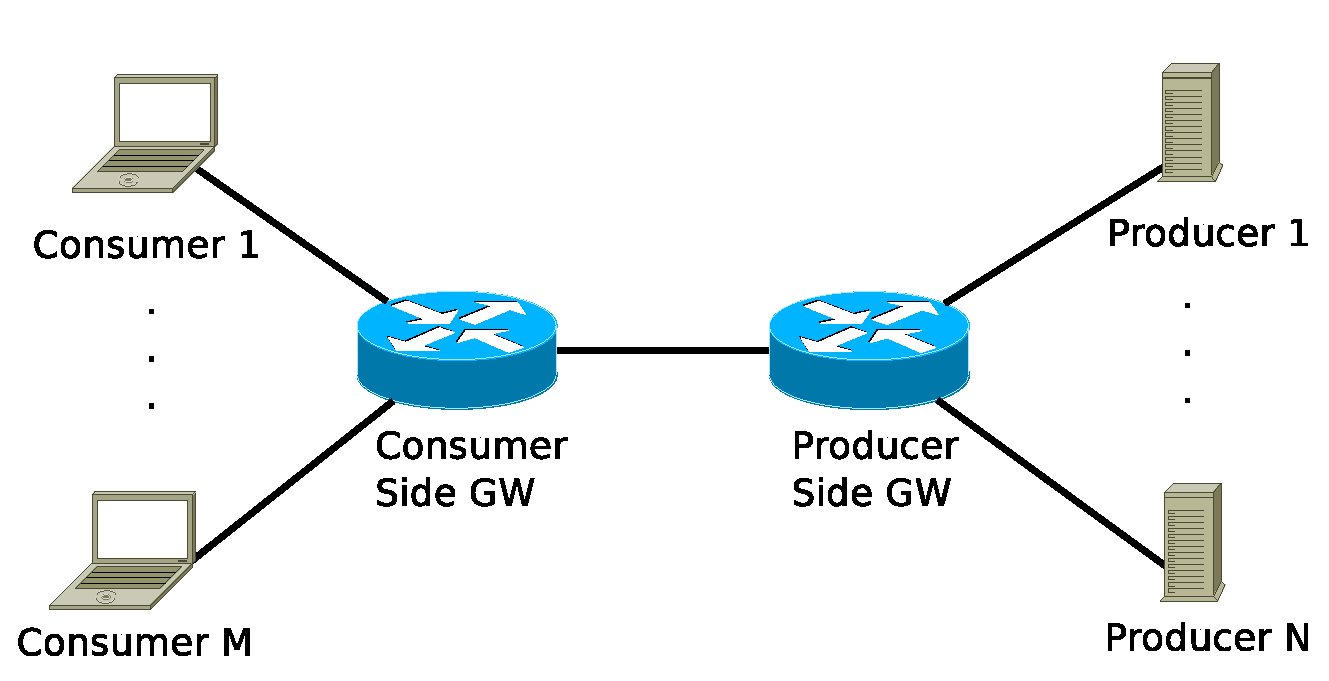
\includegraphics[width=\columnwidth]{images/testnet.eps}
\caption{Testbed network topology. $M$ consumers and $N$ producers}\label{testnet}
\end{figure}

\begin{figure}
\centering
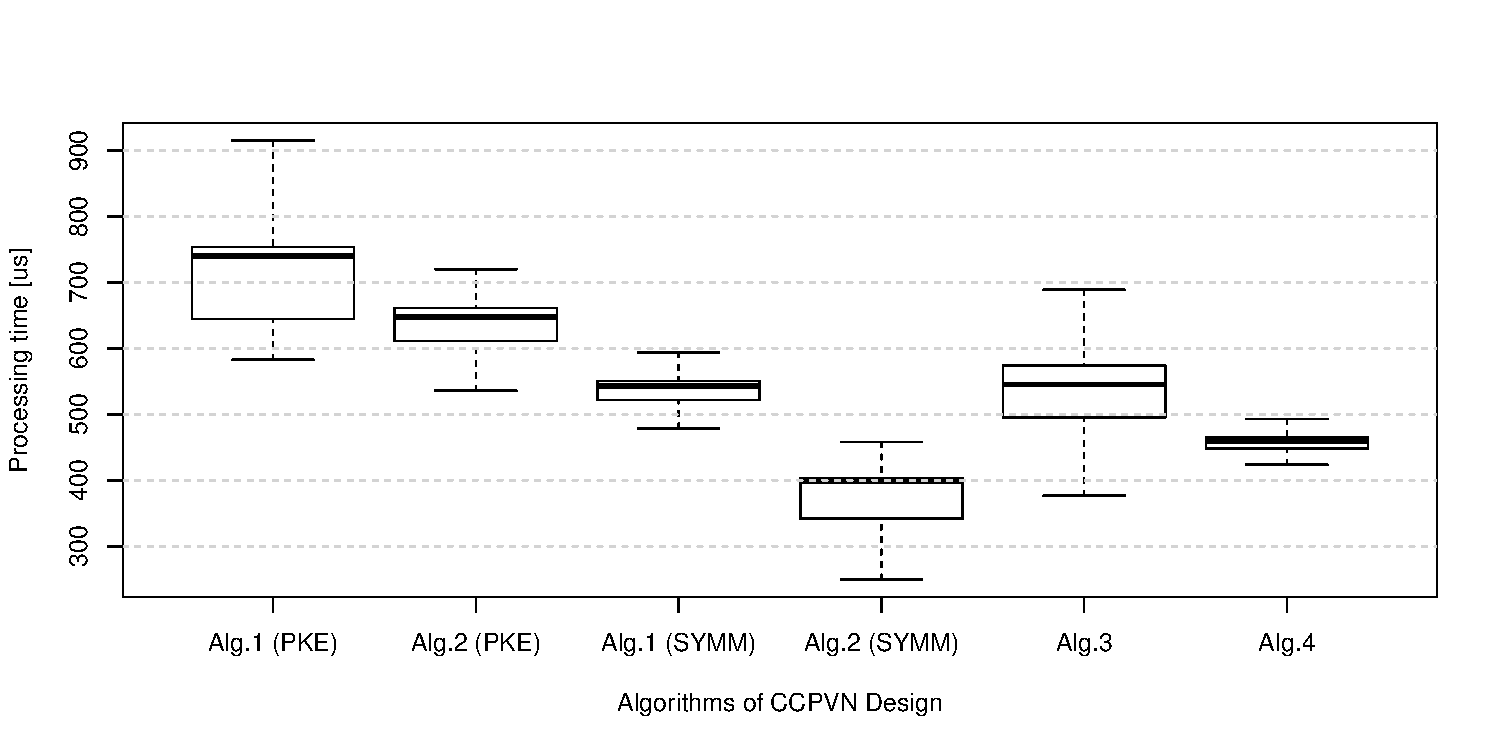
\includegraphics[width=\columnwidth]{images/times.pdf}
\caption{Execution time of the algorithms in CCVPN design}\label{times}
\end{figure}

\begin{figure}
\centering
  \subfigure[Throughput]{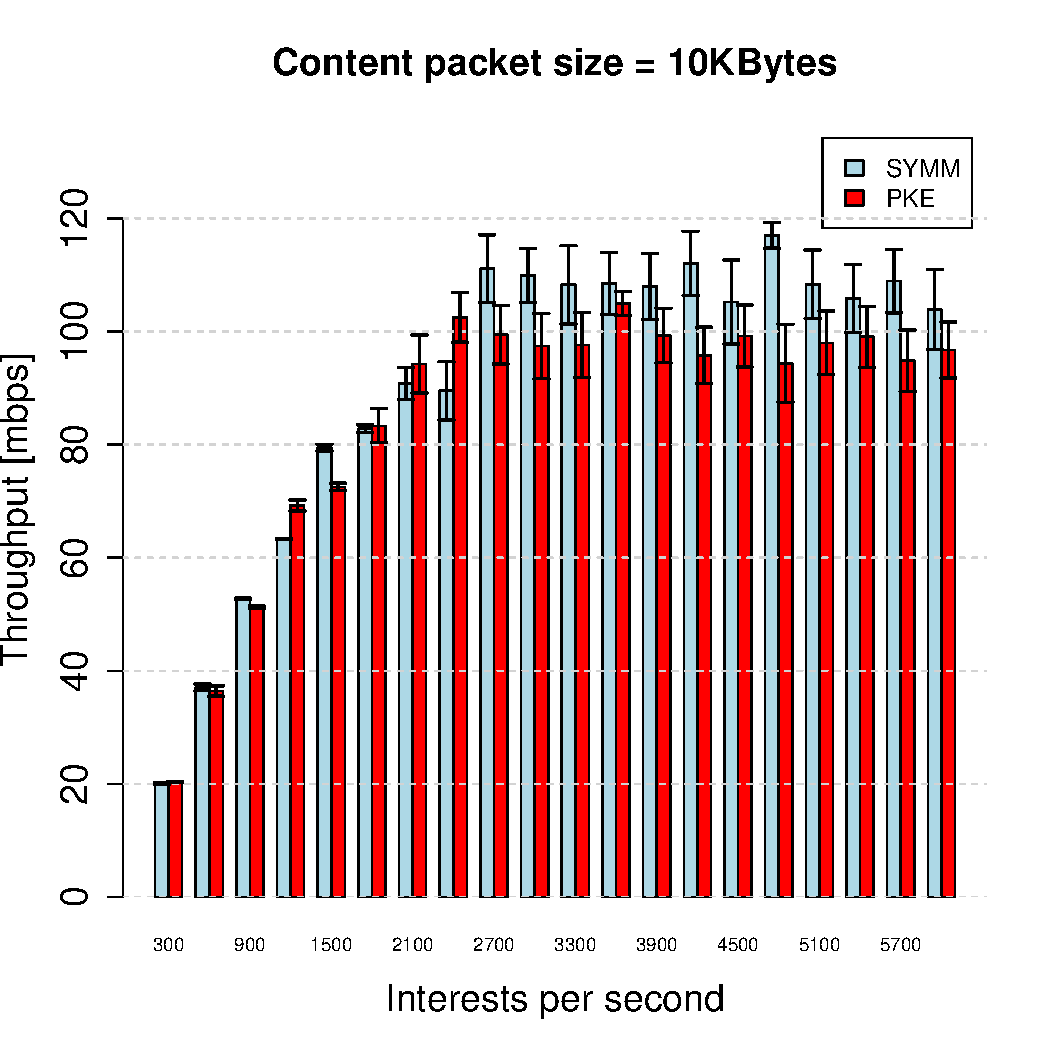
\includegraphics[width=0.8\columnwidth]{images/1_1_thput.pdf}\label{1a}}
  \hfil
  \subfigure[Avg. RTT]{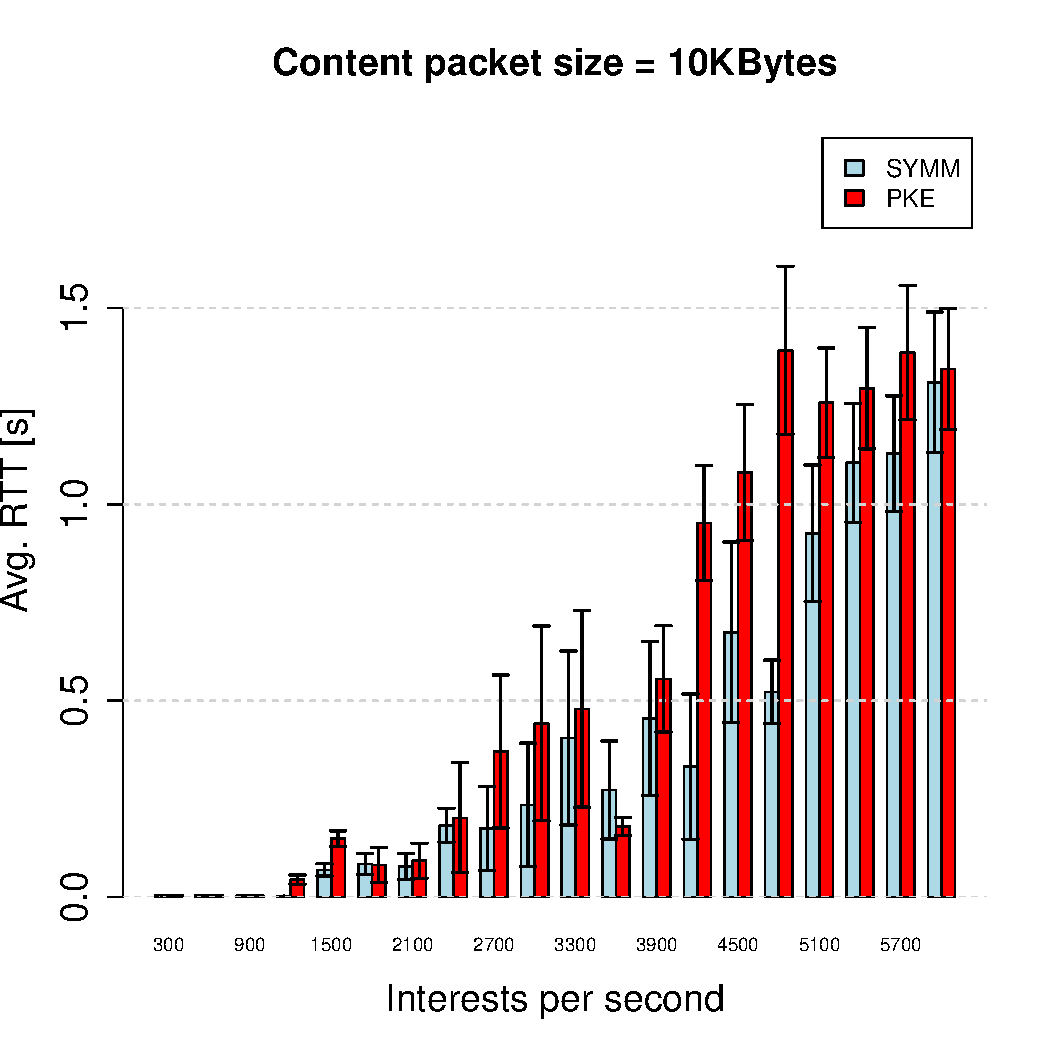
\includegraphics[width=0.8\columnwidth]{images/1_1_rtt.pdf}\label{1b}}
\caption{CCVPN performance with one consumer and one producer for increasing interest issuance rates.}\label{exp1}
\end{figure}

\begin{figure}
\centering
  \subfigure[Throughput]{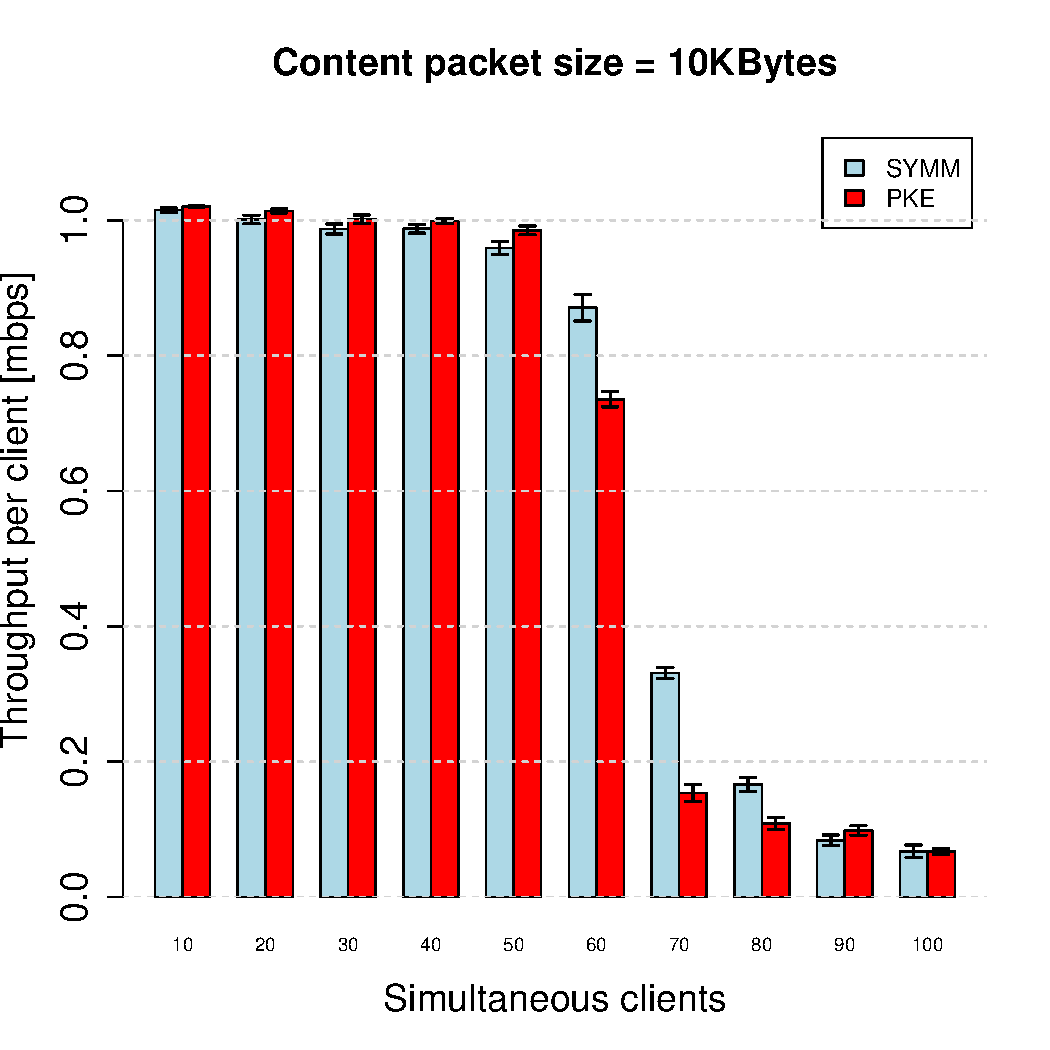
\includegraphics[width=0.7\columnwidth]{images/n_1_thput.pdf}\label{2a}}
  \hfil
  \subfigure[Avg. RTT]{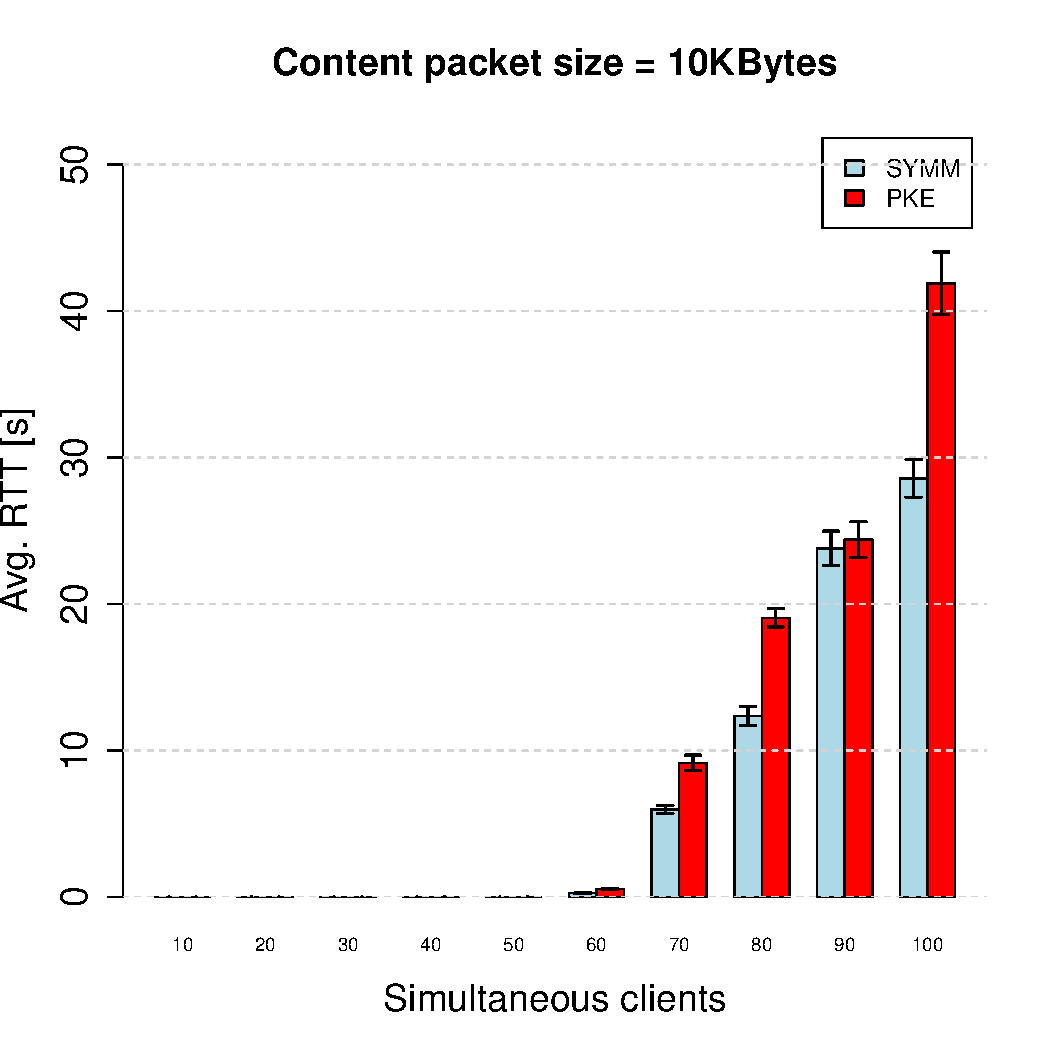
\includegraphics[width=0.7\columnwidth]{images/n_1_rtt.pdf}\label{2b}}
\caption{CCVPN performance with multiple consumers and one producer. Each consumer requests with 1 mbps rate.}\label{exp2}
\end{figure}

\begin{figure}
\centering
  \subfigure[Throughput]{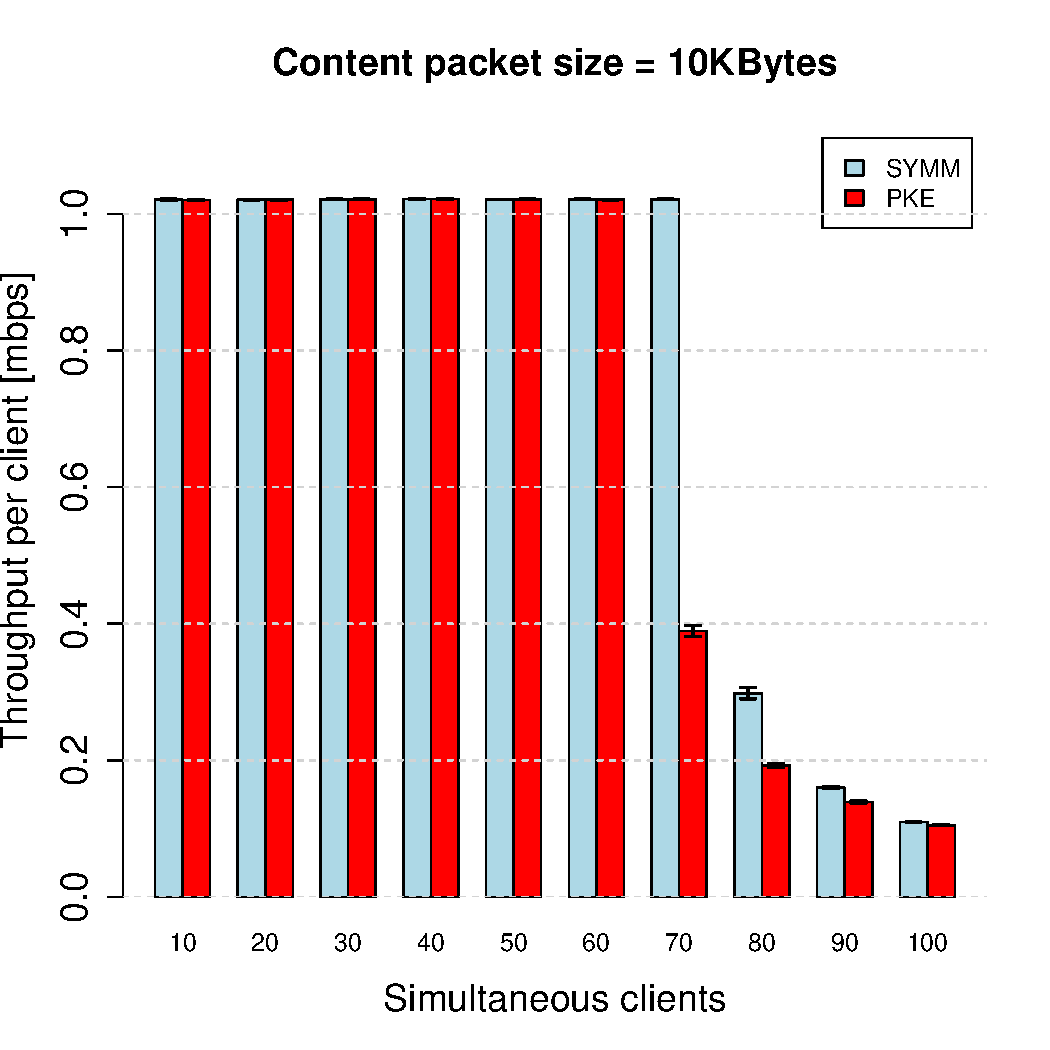
\includegraphics[width=0.7\columnwidth]{images/n_n_thput.pdf}\label{3a}}
  \hfil
  \subfigure[Avg. RTT]{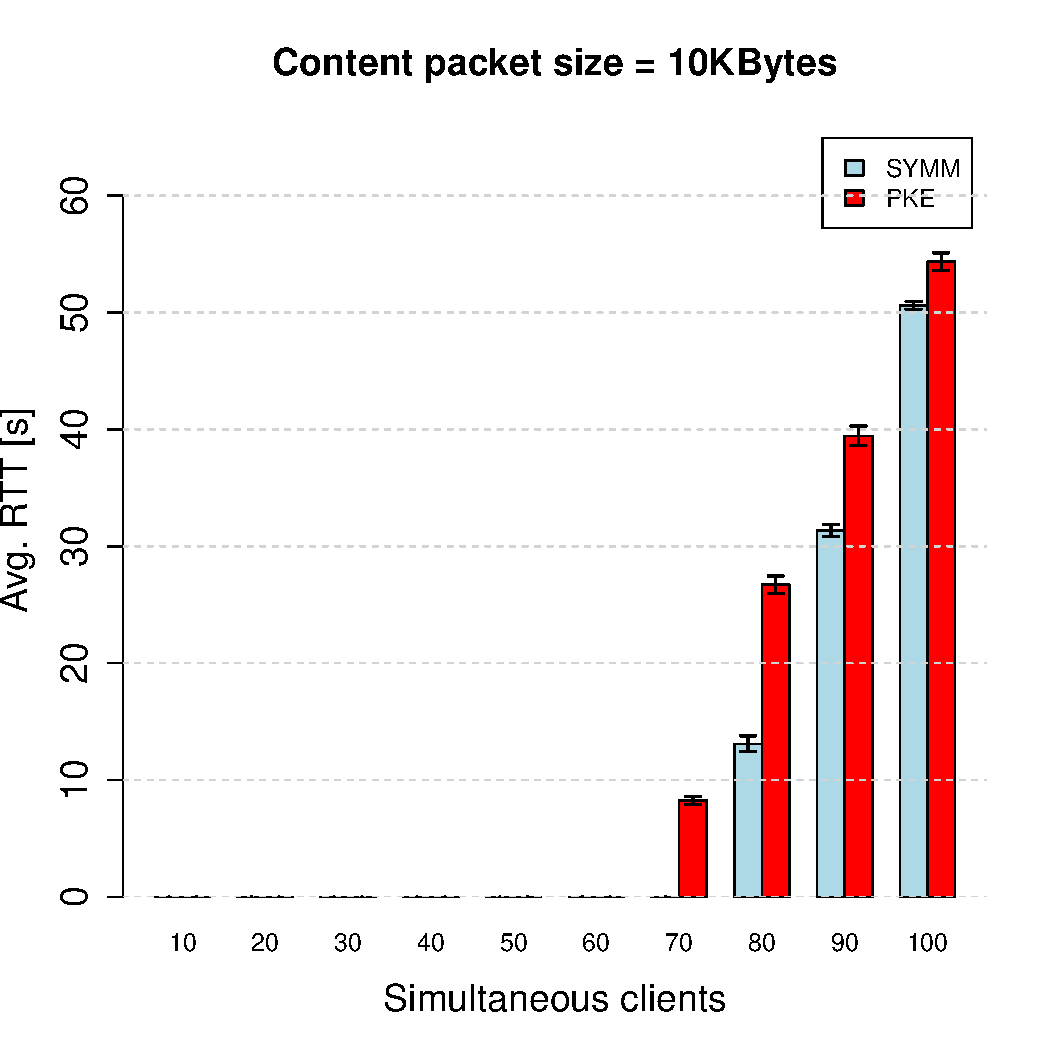
\includegraphics[width=0.7\columnwidth]{images/n_n_rtt.pdf}\label{3b}}
\caption{CCVPN performance with multiple consumers and multiple producers. Each consumer requests with 1 mbps rate.}\label{exp3}
\end{figure}


CCVPN is implemented as a network layer service running on the gateways of the private
networks that compose the VPN (see Fig.\ref{fig:ccvpn}). Our implementation uses the CCNx
software stack~\cite{CCNxGithub} and the cryptographic library Sodium~\cite{sodiumGithub}.
These are both publicly available and written in C. For the PKE version of CCVPN, we use
Sodium Sealed-Boxes~\cite{bernstein2006curve25519}, implemented over X25519 elliptic curves,
as the PKE algorithm for the interest encapsulation and decapsulation routines
(Algorithm~\ref{alg:interestEncap}, and Algorithm~\ref{alg:interestDecap} of Sec.~\ref{metho}).
AES256-GCM~\cite{dworkin2007recommendation} is used to encrypt-then-MAC content
responses (Alg.~\ref{alg:contentEnc}, and Alg.~\ref{alg:contentDec} of Sec.~\ref{metho}).
Recall that the symmetric keys used to encrypt-then-MAC the content packets are
generated and sent together with the encapsulated interest in Alg.~\ref{alg:interestEncap}.
In the symmetric key version of the design, both, interests and contents, are
encapsulated using AES256-GCM under the assumption that the gateways already share a symmetric key.

The experiments presented throughout this section were executed in an Intel
Core i7-3770 octacore CPU @3.40GHz, with 16GB of RAM, running Linux (Ubuntu 14.04LTS).
Content payload sizes were set to 10 kilobytes. On every experiment, each of the two
gateway processes (i.e., consumer side gateway process, and producer side gateway process)
were assigned as a high priority processes and each of them ran in a single core of the processor.
Fig.~\ref{times} presents box-plots for the execution times of the four algorithms
involved in CCVPN's data transmission, including both, PKE and Symmetric Key versions
for interest encapsulation and decapsulation.

With the goal of evaluating the impact of CCVPN's cryptographic overhead on the
overall network performance, we measure the network throughput and the
request-response round trip time (RTT) under different topology settings.
In our testbed network, the consumers' side and the producers' side gateways are
directly interconnected. $N$ producers are connected to the producers' domain gateway
and $M$ consumers are connected to the consumers' domain gateway, as illustrated in Fig.~\ref{testnet}.
In this topology, we consider three variations for the values of ${M,N}$:

\begin{itemize}
 \item \textbf{One consumer and one producer $[1,1]$}: We use this setting, with
 only one consumer and one producer, to slowly increase the interest issuance
 rate until we are able to determine the maximum network throughput and the
 impact on RTT as congestion increases.
 \item \textbf{Multiple consumers and one producer $[M,1]$}: In this setting we
 fix the interest issuance rate so that each consumer requests approximately $1$
 mbps of data, and we gradually increase the number of consumers in the network,
 until the throughput per consumer starts to decrease, i.e., until congestion
 starts to occur. In this setting, the interests coming from all consumers are
 served by a single producer.
 \item \textbf{Multiple consumers and multiple producers $[M,N]$}: In this experiment
 we also gradually increase the number consumers, but we increase the number of
 producers by the same amount at each round, i.e., $M=N$. The number of hosts
 (consumers and producers) is increased until congestion is observed.
\end{itemize}

It is worth to mention that, in all of the considered settings, every interest
is a unique request for a unique piece of content. Therefore, the experiments
present the throughput and RTT in the worst case scenario of a CCN, i.e., when
there is no content caching in the gateway.

Fig.~\ref{exp1} shows the the network performance when $[M,N]=[1,1]$ as the
consumer's request rate increases. The network achieves a maximum throughput of
$100$ mbps in the PKE version and a slightly higher throughput of $110$ mbps in
the symmetric key version. Conversely, the average RTT per message starts to
increase as the interest issuance rate approaches the maximum network throughput,
as a signal of congestion in the routers.

The results for multiple consumers requesting to a single producer ($[M,1]$) are
depicted in Fig.~\ref{exp2}. In this setting, each consumer receives close to the
requested throughput ($1$ mbps) when less than $50$ clients are requesting contents at
the same time. With more than $60$ clients the Avg. RTT starts to increase due to
congestion, and the average throughput experienced by each client is gradually reduced.

Since in CCN the consumer signs every content, the congestion presented in
Fig.~\ref{exp2} might be influenced by the overhead of having a single producer
signing an enormous number of interests, in addition to the gateways' cryptographic overhead.
To evaluate that effect in Fig.~\ref{exp3}, we show the average throughput and RTT
in the scenario with $[M,N]$ consumers and producers, where $M=N$ and each consumer
requests from a specific producer. In such scenario, we see that the results are
slightly better. The network offers the requested throughput ($1$ mbps per client)
with up to $60$ nodes, in PKE mode, and $70$ nodes, in symmetric key mode.


\subsection{Discussion}

CCVPN  exhibits moderately good results with respect to the network load capacity, considering the overheads implied by the deployment of secure tunnels over the CCN architecture.
With gateways' processes running each on a single core of a single processor, the VPN was capable of providing reasonable throughput to up to 70 clients.
This performance results are a lower bound that can be improved in several ways, among which we highlight:

\begin{enumerate}
 \item \textbf{Implementation optimization:} The CCNx software stack is an ongoing research project, and as such, the implementation focus on functionality rather than performance.
 We believe that the results presented in this section could be significantly improved by optimizations that do not rely exclusively on CCVPN design, but also in CCNx software.
 \item \textbf{Distributed and parallel processing:} In a real deployment scenario, we expect that a large scale organization, which wants to implement a VPN service, to have dedicated network devices running
 the gateway service, possibly in multiple cores. Moreover, it is not hard to imagine multiple VPN gateways sharing the load in a large organization.
 In such scenarios, we expect the network capacity (in terms throughput or number of simultaneous consumers) to scale linearly with the increase of dedicated computational resources.
 \item \textbf{Caching:} Content caching is a major advantage of ICNs when compared to the IP model. In our experiments we wanted to evaluate the worst case scenario. Therefore, clients always request different contents
 and content caching does not happen. In a real world deployment, contents that are popular (inside the VPN) would be potentially cached, significantly increasing the throughput and reducing the RTT.

\end{enumerate}


\section{Conclusion}\label{sec:conclusion}
We presented the design, implementation, and assessment of CCVPN, a scheme and
protocol for building secure and private tunnels in CCN. CCVPN allows two namespaces
to be bridged by a tunnel across a public network. Unlike point-to-point tunnels,
such as those enabled by secure session protocols, CCVPN allows many consumers
to share the tunnel to access the private namespace. CCVPN is designed with efficiency
in mind: public-key cryptographic operations are kept to a minimum during normal
operation; symmetric-key packet encapsulation algorithms are used to marshall
packets between gateways. Our experimental evidence indicate that CCVPN offers
modest performance in the presence of a variable number of consumers and producers.
The results suggest that CCVPN could be deployed for private namespace tunneling
in real world CCN deployments.

For future work, we plan to implement the CCNxKE protocol from~\cite{ccnxke} as a
way to bootstrap symmetric-key tunnels in CCVPN. We will also integrate CCVPN into
real world testbeds to assess its performance for real-world applications. These
include video streaming and large-scale content dissemination applications. Finally,
we plan to investigate countermeasures to DoS attacks on CCVPN, such as puzzles for tunnel establishment.

\ifCLASSOPTIONcaptionsoff
  \newpage
\fi

\tiny

\bibliographystyle{IEEEtran}
\bibliography{references}

% \begin{IEEEbiography}[{\includegraphics[width=1in,height=1.25in,clip,keepaspectratio]{picture}}]{John Doe}
% \blindtext
% \end{IEEEbiography}

\end{document}
